%--------------------------------------------------------------
% thesis.tex 
%--------------------------------------------------------------
% Corso di Laurea in Informatica 
% http://if.dsi.unifi.it/
% @Facolt\`a di Scienze Matematiche, Fisiche e Naturali
% @Universit\`a degli Studi di Firenze
%--------------------------------------------------------------
% - template for the main file of Informatica@Unifi Thesis 
% - based on Classic Thesis Style Copyright (C) 2008 
%   Andr\'e Miede http://www.miede.de   
%--------------------------------------------------------------
\documentclass[twoside,openright,titlepage,fleqn,
	headinclude,12pt,a4paper,BCOR=5mm,footinclude]{scrbook}
%--------------------------------------------------------------
\newcommand{\myItalianTitle}{studio e sperimentazione del microkernel seL4\xspace}
\newcommand{\myEnglishTitle}{Studying and experimenting with the seL4 microkernel\xspace}
% use the right myDegree option
\newcommand{\myDegree}{Corso di Laurea in Informatica\xspace}
%\newcommand{\myDegree}{
	%Corso di Laurea Specialistica in Scienze e Tecnologie 
	%dell'Informazione\xspace}
\newcommand{\myName}{Elia Matteini\xspace}
\newcommand{\myProf}{Rosario Pugliese\xspace}
%\newcommand{\myOtherProf}{Correlatore\xspace}
%\newcommand{\mySupervisor}{Nome Cognome\xspace}
\newcommand{\myFaculty}{
	Scuola di Scienze Matematiche, Fisiche e Naturali\xspace}
\newcommand{\myUni}{\protect{
	Universit\`a degli Studi di Firenze}\xspace}
\newcommand{\myLocation}{Firenze\xspace}
\newcommand{\myTime}{Anno Accademico 2022-2023\xspace}
\newcommand{\myVersion}{Version 0.1\xspace}
%--------------------------------------------------------------
\usepackage[italian]{babel}
\usepackage[utf8]{inputenc} %\usepackage[latin1]{inputenc}
\usepackage[T1]{fontenc} 
\usepackage[scaled]{helvet} %\usepackage[default]{nome_font}
\usepackage[square,numbers]{natbib} 
\usepackage[fleqn]{amsmath}  
\usepackage{ellipsis}
\usepackage{listings}
\usepackage{subfig}
\usepackage{caption}
\usepackage{appendix}
\usepackage{siunitx}
%--------------------------------------------------------------
\usepackage{dia-classicthesis-ldpkg}
%\usepackage{classicthesis}
%--------------------------------------------------------------
% Options for classicthesis.sty:
% tocaligned eulerchapternumbers drafting linedheaders 
% listsseparated subfig nochapters beramono eulermath parts 
% minionpro pdfspacing
\usepackage[eulerchapternumbers,linedheaders,subfig,beramono,eulermath,
parts,dottedtoc]{classicthesis}
%--------------------------------------------------------------
\newlength{\abcd} % for ab..z string length calculation
% how all the floats will be aligned
\newcommand{\myfloatalign}{\centering} 
\setlength{\extrarowheight}{3pt} % increase table row height
\captionsetup{format=hang,font=small}
%--------------------------------------------------------------
% Layout setting
%--------------------------------------------------------------
\usepackage{geometry}
\geometry{
	a4paper,
	ignoremp,
	bindingoffset = 1cm, 
	textwidth     = 13.5cm,
	textheight    = 21.5cm,
	lmargin       = 3.5cm, % left margin
	tmargin       = 4cm    % top margin 
}

\lstset{
  	%frame=tb,
	language=Matlab,
  	aboveskip=3mm,
  	belowskip=3mm,
  	showstringspaces=false,
  	columns=flexible,
  	basicstyle={\small\ttfamily},
  	numbers=none,
  	breaklines=true,
  	breakatwhitespace=true,
  	tabsize=3
}
\usepackage{dirtree}
\usepackage{url}
\usepackage{float}
%--------------------------------------------------------------
\begin{document}
\frenchspacing
\raggedbottom
\pagenumbering{roman}
\pagestyle{plain}
\sloppy
%--------------------------------------------------------------
% Frontmatter
%--------------------------------------------------------------
%--------------------------------------------------------------
% titlepage.tex (use thesis.tex as main file)
%--------------------------------------------------------------
\begin{titlepage}
	\begin{center}
   	\large
      \hfill
      \vfill
      \begingroup
         \includegraphics[scale=0.15]{logo/LOGO}\\
%			\spacedallcaps{\myUni} \\ 
			\myFaculty \\
			\myDegree \\ 
			\vspace{0.5cm}
         \vspace{0.5cm}    
         Tesi di Laurea    
      \endgroup 
      \vfill 
      \begingroup
      	\color{Maroon}\spacedallcaps{\myItalianTitle} \\ $\ $\\
      	\spacedallcaps{\myEnglishTitle} \\ 	
	\bigskip
      \endgroup
      \spacedlowsmallcaps{\myName}
      \vfill 
      \vfill
      Relatore: \emph{\myProf}\\
      %Correlatore: \emph{Correlatore}\\
      \vfill
      \vfill
      \myTime
      \vfill                      
	\end{center}        
\end{titlepage}   
%--------------------------------------------------------------
% back titlepage
%--------------------------------------------------------------
   \newpage
	\thispagestyle{empty}
	\hfill
	\vfill
	\noindent\myName: 
	\textit{\myItalianTitle,} 
	\myDegree, \textcopyright\ \myTime
%--------------------------------------------------------------
% back titlepage end
%--------------------------------------------------------------
\pagestyle{scrheadings}
%--------------------------------------------------------------
% Mainmatter
%--------------------------------------------------------------
\pagenumbering{arabic}
% use \cleardoublepage here to avoid problems with pdfbookmark
%\include{intro} % use \myChapter command instead of \chapter
\tableofcontents
%\listoffigures
\cleardoublepage
\thispagestyle{empty}
\begin{flushright}
\null\vspace{\stretch {1}}
\emph{"Inserire citazione" \break --- Inserire autore citazione} \vspace{\stretch{2}}\null
\end{flushright}
\setcounter{chapter}{-1}
\renewcommand{\thechapter}{I}
\chapter{Introduzione}
In questa introduzione sarà presente una prima parte che andrà a dare le conoscenze di base minime per comprendere cosa sia un sistema operativo e una piccola classificazione, dopodiché seguiranno la descrizione di alcuni concetti che sono fondamentali per comprendere il resto dell'elaborato.

\section{Cos'è un sistema operativo}
Un sistema operativo (SO) è un insieme di software che gestisce le risorse hardware e software di un sistema di elaborazione fornendo servizi agli applicativi utente.\\
In un computer quindi il sistema operativo fornisce l'unica interfaccia diretta con l'hardware e in quanto tale ha un accesso esclusivo con il massimo dei privilegi detto \textit{kernel mode}. Questo comporta che una vulnerabilità all'interno del sistema operativo può portare a gravi conseguenze per l'integrità e la sicurezza del sistema, inoltre qualche malintenzionato potrebbe approfittare di questo bug per trarne profitto.
Uno degli obiettivi principali di un SO è quindi quello di garantire la sicurezza, ulteriore scopo è l'efficienza: un buon sistema operativo deve saper sfruttare al meglio tutte le risorse che ha a disposizione, dalla gestione della memoria per sfruttare al meglio lo spazio alla schedulazione dei processi per ottimizzare i tempi di esecuzione. Come ultimo obiettivo, ma non per questo meno rilevante, deve rendere il più semplice possibile l'utilizzo del dispositivo su cui è installato.
Dalla definizione di SO data a inizio capitolo possiamo isolare una specifica parte di codice che è quella che permette al software di interfacciarsi con l'hardware, quindi l'accesso e la gestione delle risorse di un dispositivo, questa specifica parte si chiama \textit{kernel} che come suggerisci il nome (nocciolo dall'inglese) rappresenta la parte centrale di un sistema operativo su cui tutto il resto si appoggia.
\newpage

\section{Microkernel e kernel monolitici}
Esistono vari modelli strutturali per i sistemi operativi: monolitici, modulari, a livelli, microkernel ed ibridi, ad oggi i più diffusi sono gli ibridi, che combinano i vari modelli tra di loro, ma che in gran parte si basano su sistemi monolitici i quali consistono di un unico file binario statico al cui interno sono definite tutte le funzionalità del kernel e che viene eseguito in un unico spazio di indirizzi, questo comporta dei vantaggi: 
\begin{itemize}
	\item[-] efficienza $\rightarrow$ motivo principale per cui la maggior parte dei sistemi operativi ancora si basano su kernel in gran parte monolitici, lavorando nello stesso spazio di indirizzi e gestendo tutto attraverso chiamate a procedura il SO risulterà molto reattivo e performante
	\item[-] semplicità $\rightarrow$ in quanto non ha una vera e  propria strutturazione ma il codice è tutto in un unico file binario risulta chiaramente più semplice da progettare anche se poi l'implementazione risulta difficile
\end{itemize} 
d'altra parte ha anche degli svantaggi: 
\begin{itemize}
	\item[-] inserimento di un nuovo servizio $\rightarrow$ questo richiede la ricompilazione del kernel, quindi non permette l'inserimento di un nuovo servizio a runtime (problema risolto nei modelli ibridi)
	\item[-] dimensione $\rightarrow$ dovendo gestire tutte le principali funzionalità del sistema operativo il kernel sarà composto da milioni di righe di codice sorgente (MSLOC - linux ha circa 20MSLOC) e questo porta direttamente al successivo grosso svantaggio
	\item[-] sicurezza $\rightarrow$ maggiore è il numero di righe di codice maggiore sarà il numero di possibili bug, essendo tutto il codice eseguito nello stesso spazio di indirizzi un bug rischia di far 	bloccare l'intero sistema anche se il problema è molto piccolo e isolato a una minima funzione del kernel.
\end{itemize}
All'estremo opposto troviamo i \textit{microkernel} che sono composti da un kernel ridotto al minimo indispensabile, che comprende la gestione della memoria, dei processi e della CPU, le comunicazioni tra processi (IPC) e l'hardware di basso livello, mentre tutto il resto deve essere gestito da server (deamon) che operano sopra al kernel, quindi in spazi di indirizzi separati.\\ I microkernel sono spesso usati in sistemi embedded in applicazioni mission critical di automazione robotica o di medicina, a causa del fatto che i componenti del sistema risiedono in aree di memoria separate, private e protette.\\
Anche questo modello ha dei vantaggi:
\begin{itemize}
	\item[-] flessibilità $\rightarrow$ l'inserimento di un nuovo servizio avviene al di sopra del kernel quindi in qualsiasi momento è possibili aggiungere o togliere servizi senza dover modificare il kernel.
	\item[-] sicurezza $\rightarrow$ minore quantità di codice eseguita in kernel mode (quindi minore quantità di bug e minore superficie attaccabile) maggiore è la sicurezza del sistema, inoltre i servizi sono lavorano in uno spazio di indirizzi differente da quello del kernel di conseguenza se un server (su cui viene eseguito un servizio) smette di funzionare tutto il resto del sistema continua a funzionare normalmente e si potrà procedere a riavviare quel singolo servizio
	\item[-] semplicità $\rightarrow$ essendo il codice composto da giusto qualche decina di migliaia di righe di codice (KSLOC) risulta molto più facile da scrivere
\end{itemize}
e dall'altro lato ha un grande svantaggio:
\begin{itemize}
	\item[-] efficienza $\rightarrow$ dato che ogni servizio gira a livello utente l'utilizzo di uno qualsiasi di questi richiede il ricorso a chiamate di sistema che rallentano fortemente l'esecuzione di ogni operazione, motivo principale per cui ancora oggi i sistemi operativi si basano in gran parte su sistemi monolitici.
\end{itemize}

\begin{figure}[h]
  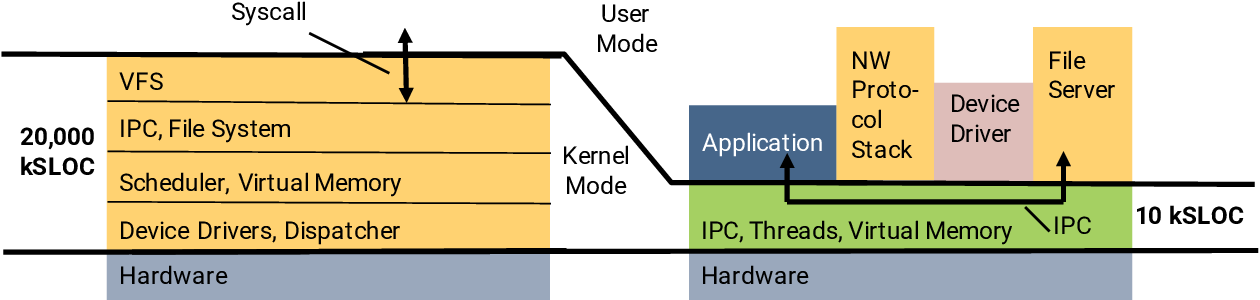
\includegraphics[width=\linewidth]{img/MonolithicVSmicrokernel.png}
  \caption{Kernel monolitici (sinistra) VS microkernel (destra)}
  \label{fig:MonolithicVSmicrokernel}
\end{figure}
\newpage

\section{Scheduling}
Proseguendo la lettura verrà nominato lo scheduling: solitamente con il solo termine scheduling si intende quello a breve termine della CPU, cioè la funzionalità che determina quale tra i processi (thread) in attesa della CPU la otterranno, ci sono vari metodi che si differenziano per modalità e prestazioni, gli algoritmi che traducono questi metodi si chiamano politiche di scheduling.
Una particolare politica di scheduling rilevante per questo testo è Round Robin o scheduling circolare: consiste nel determinare una quantità di tempo (time slice) nella quale il processo ottiene la CPU al termine del quale il processo viene interrotto e inserito infondo alla lista dei processi in attesa, in questo modo tutti i processi ottengono la CPU per al più un tempo massimo stabilito ed è anche possibile stabilire un tempo massimo di attesa che un processo dovrà attendere in base a quanti processi lo precedono.

\section{Hypervisor}
Un \textit{hypervisor}, chiamato anche virtual machine monitor (VMM), è un tipo di sotware/firmware che permette di creare ed eseguire macchine virtuali. Un computer sul quale un hypervisor esegue una o più macchine virtuali prende il nome di host machine mentre le singole macchina virtuali prenderanno il nome di guest machine, su ognuna di queste è possibile far girare un sistema operativo diverso che eseguirà la maggior parte delle istruzioni direttamente sulle risorse hardware virtualizzate rese disponibili dall'hypervisor.
\renewcommand{\thechapter}{\arabic{chapter}}
\chapter{Background}
In questa introduzione sarà presente una prima parte che andrà a dare le conoscenze di base minime per comprendere cosa sia un sistema operativo e una piccola classificazione di essi, dopodiché seguiranno la descrizione di alcuni concetti che sono fondamentali per comprendere il resto dell'elaborato.

\section{Cos'è un sistema operativo}
Un sistema operativo (SO) è un software che gestisce le risorse \textit{hardware} e \textit{software} di un sistema di elaborazione fornendo servizi agli applicativi utente.

In un computer quindi esso fornisce l'unica interfaccia diretta con l'\textit{hardware} e in quanto tale ha un accesso esclusivo con il massimo dei privilegi detto \textit{kernel mode}. Questo comporta che una vulnerabilità all'interno del sistema operativo può portare a gravi conseguenze per l'integrità e la sicurezza del sistema, inoltre qualche malintenzionato potrebbe approfittare di questo \textit{bug} per trarne profitto.

Uno degli obiettivi principali di un SO è quindi quello di garantire la sicurezza; ulteriore scopo è l'efficienza: un buon sistema operativo deve saper sfruttare al meglio tutte le risorse che ha a disposizione, dalla gestione della memoria per sfruttare al meglio lo spazio alla schedulazione dei processi per ottimizzare i tempi di esecuzione. Come ultimo obiettivo, ma non per questo meno rilevante, deve rendere il più semplice possibile l'utilizzo del dispositivo su cui è installato.
All'interno si un di SO possiamo isolare una specifica parte di codice che è quella che permette al \textit{software} di interfacciarsi con l'\textit{hardware}, quindi l'accesso e la gestione delle risorse di un dispositivo. Questa specifica parte si chiama \textit{kernel}, che come suggerisce il nome (nocciolo dall'inglese), rappresenta la parte centrale di un sistema operativo su cui tutto il resto si appoggia.
\newpage

\section{Architettura software di un sistema operativo}
Esistono vari modelli strutturali per i sistemi operativi: monolitici, modulari, a livelli, microkernel ed ibridi. Ad oggi i più diffusi sono gli ibridi, che combinano i vari modelli tra di loro, ma che in gran parte si basano su sistemi monolitici. Quest'ultimi consistono di un unico file binario statico al cui interno sono definite tutte le funzionalità del \textit{kernel} e che viene eseguito in un unico spazio di indirizzi. Tutto ciò comporta dei vantaggi: 
\begin{itemize}
	\item[-] efficienza: motivo principale per cui la maggior parte dei sistemi operativi ancora oggi si basano su \textit{kernel} in gran parte monolitici, lavorando nello stesso spazio di indirizzi e gestendo tutto attraverso chiamate a procedura il SO risulterà molto reattivo e performante;
	\item[-] semplicità: in quanto non ha una vera e  propria strutturazione, bensì il codice è tutto in un unico file binario, risulta chiaramente più semplice da progettare anche se poi l'implementazione risulta difficile.
\end{itemize} 
D'altra parte ha anche degli svantaggi: 
\begin{itemize}
	\item[-] inserimento di un nuovo servizio: questo richiede la ricompilazione del \textit{kernel}, quindi non permette l'inserimento di un nuovo servizio a \textit{runtime} (problema risolto nei modelli ibridi);
	\item[-] dimensione: dovendo gestire tutte le principali funzionalità del sistema operativo, il \textit{kernel} sarà composto da milioni di righe di codice sorgente (MSLOC - linux ha circa 20MSLOC) e questo porta direttamente al successivo grosso svantaggio;
	\item[-] sicurezza: maggiore è il numero di righe di codice maggiore sarà il numero di possibili \textit{bug}; essendo tutto il codice eseguito nello stesso spazio di indirizzi un \textit{bug} rischia di far bloccare l'intero sistema anche se il problema è molto piccolo e isolato a una minima funzione del kernel.
\end{itemize}

All'estremo opposto troviamo i microkernel che sono composti da un \textit{kernel} ridotto al minimo indispensabile, che comprende la gestione della memoria, dei processi e della CPU, le comunicazioni tra processi (IPC) e l'hardware di basso livello; tutto il resto deve essere gestito da server (\textit{daemon}) che operano sopra al kernel, quindi in spazi di indirizzi separati.

I microkernel sono spesso usati in sistemi \textit{embedded}, in applicazioni \textit{mission critical} di automazione robotica o di medicina, a causa del fatto che i componenti del sistema risiedono in aree di memoria separate, private e protette \cite{kernelWikipedia}.

Anche questo modello ha dei vantaggi:
\begin{itemize}
	\item[-] flessibilità: l'inserimento di un nuovo servizio avviene al di sopra del \textit{kernel} quindi in qualsiasi momento è possibile aggiungere o togliere servizi senza dover modificare il \textit{kernel};
	\item[-] sicurezza: minore quantità di codice eseguita in \textit{kernel} mode (quindi minore quantità di \textit{bug} e minore superficie attaccabile) quindi maggiore sicurezza del sistema; inoltre i servizi lavorano in uno spazio di indirizzi differente da quello del \textit{kernel} di conseguenza se un server (su cui viene eseguito un servizio) smette di funzionare tutto il resto del sistema continua a funzionare normalmente e si potrà procedere a riavviare quel singolo servizio;
	\item[-] semplicità: essendo il codice composto da qualche decina di migliaia di righe di codice (KSLOC) risulta molto più facile da scrivere.
\end{itemize}
Dall'altro lato ha un grande svantaggio:
\begin{itemize}
	\item[-] efficienza: dato che ogni servizio è eseguito a livello utente, l'utilizzo di uno qualsiasi di questi richiede il ricorso a chiamate di sistema che rallentano fortemente l'esecuzione di ogni operazione, motivo principale per cui ancora oggi i sistemi operativi si basano in gran parte su sistemi monolitici.
\end{itemize}
In Figura~\ref{fig:MonolithicVSmicrokernel} si possono vedere in maniera schematica le differenza tra \textit{kernel} monolitici e mircrokernel.

\begin{figure}[h]
  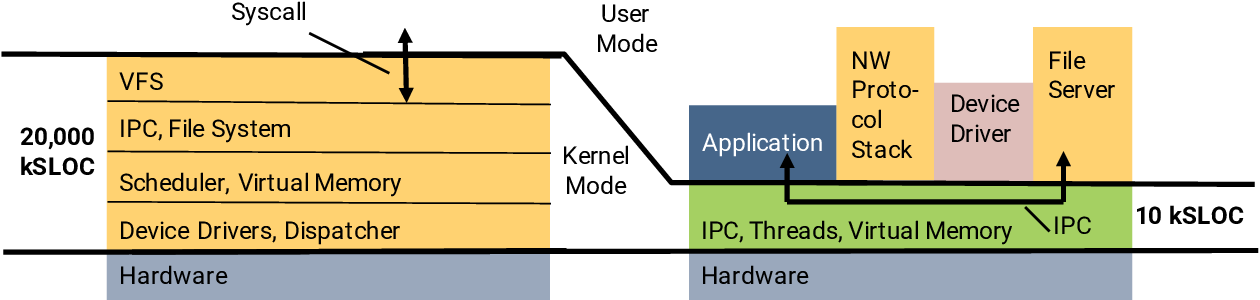
\includegraphics[width=\linewidth]{img/MonolithicVSmicrokernel.png}
  \caption{Kernel monolitici (sinistra) VS Microkernel (destra)}
  \label{fig:MonolithicVSmicrokernel}
\end{figure}
\newpage

\section{Scheduling della CPU}
Solitamente con il solo termine \textit{scheduling} si intende quello a breve termine della CPU, cioè la funzionalità che determina quale tra i processi (\textit{thread}) in attesa della CPU la otterranno. Chiaramente ci sono vari metodi per fare ciò, che prendono il nome di politiche di \textit{scheduling}, i quali si differenziano per modalità e prestazioni. Gli algoritmi che traducono questi metodi si chiamano algoritmi di \textit{scheduling}.

Una particolare politica di \textit{scheduling} rilevante per questo testo è \textit{Round Robin} o \textit{scheduling circolare}: consiste nel determinare un quanto di tempo (\textit{time slice}) nella quale i processi ottengono la CPU. Una volta esaurito questo tempo il processo viene interrotto e inserito in fondo alla coda dei pronti. In questo modo tutti i processi ottengono la CPU per un tempo massimo stabilito; inoltre è possibile stabilire il tempo di attesa prima dell'esecuzione di ciascun processo in base al numero di processi che lo precedono.

\section{Memoria virtuale}
Un altro concetto fondamentale quando si parla di sistemi operativi è la gestione della memoria. Il SO deve garantire che ogni programma abbia a disposizione la giusta quantità di memoria necessaria per l'esecuzione, ed inoltre ognuno di essi deve accedere solo alla memoria a lui riservata. Un meccanismo adottato che accomuna quanto appena detto è quello di memoria virtuale.

La memoria virtuale è un meccanismo che permette di simulare uno spazio di memoria centrale (memoria primaria) maggiore di quello fisicamente presente o disponibile, dando l'illusione all'utente di un enorme quantitativo di memoria. Questa tecnica porta con sé diversi vantaggi: uno tra questi la sicurezza dovuta all'isolamento della memoria; la possibilità di condivisione di alcune pagine di memoria tra più processi (es: le pagine contenenti le librerie possono essere usate in contemporanea da più processi senza conflitti) e infine l'ultimo ma allo stesso tempo il principale vantaggio: avere a disposizione molta più memoria centrale di quella che in realtà è disponibile. 

Giustamente viene da chiedersi com'è possibile tutto ciò e il meccanismo alla base è quello di utilizzare una memoria ausiliaria, solitamente la memoria di massa, per allocare una certa parte di memoria che non è stata utilizzata recentemente. Nel momento in cui viene richiesto nuovamente la porzione di dati salvati nella memoria ausiliaria (oppure si libera spazio nella memoria centrale) i dati relativi vengono prelevati e copiati nuovamente in memoria centrale, questo processo prende il nome di \textit{swapping}. 

In presenza di memoria virtuale quindi non parleremo semplicemente di indirizzi di memoria ma avremo una differenziazione tra indirizzi logici e indirizzi fisici. I programmi lavoreranno solo con indirizzi logici (quindi viene anche facilitata la programmazione) e poi a livello di CPU avverrà un processo di traduzione negli indirizzi fisici.

\section{Hypervisor}
Un \textit{hypervisor}, chiamato anche \textit{virtual machine monitor} (VMM), è un tipo di \textit{sotware/firmware} che permette di creare ed eseguire macchine virtuali. Un computer sul quale un \textit{hypervisor} esegue una o più macchine virtuali prende il nome di \textit{host machine}, mentre le singole macchina virtuali prendono il nome di \textit{guest machine}. Su ognuna è possibile eseguire un sistema operativo (anche diverso) che eseguirà la maggior parte delle istruzioni direttamente sulle risorse \textit{hardware} virtualizzate rese disponibili dall'\textit{hypervisor}.
\include{Chapters/sel4}
\chapter{Sperimentazione di seL4}
In questo capitolo viene affrontato il \textit{focus} della tesi, cioè la sperimentazione di \textit{seL4}. Seguiranno tutti gli \textit{step} che sono stati messi in pratica durante questa fase dello studio del sistema: dall'installazione di un sistema operativo in cui poter simulare \textit{seL4}, fino allo sperimentare con mano le varie funzionalità. Ovviamente questo ha richiesto un approfondimento più tecnico e specifico, rispetto a quanto realizzato finora, di alcuni aspetti come la gestione della memoria fisica e virtuale, l'IPC, ecc.

\section{Prerequisiti}
Come prima cosa ho installato \textit{VirtualBox} (macchina virtuale) sul mio portatile in quanto, come consigliato dalle linee guida fornite da \textit{Trustworthy System} (TS), è ottimale lavorare in ambiente Linux. Inizialmente ho pensato di utilizzare una macchina virtuale con Linux, così da lasciare inalterato il mio computer e comunque avere a disposizione un sistema operativo Linux su cui operare. Andando avanti con il \textit{set-up} del sistema per iniziare a lavorare su seL4, ho però incontrato una prima difficoltà: lo spazio nel portatile non era purtroppo adeguato e la macchina virtuale, considerando il sistema operativo e l'installazione dei vari prerequisiti per poter far girare il \textit{microkernel}, cominciava ad occupare una quantità di memoria non trascurabile. Ho di conseguenza dovuto cercare un'alternativa. Per sopperire al problema, mi sono procurato un SSD su cui sono andato a copiare la partizione creata in \textit{VirtualBox}, continuando la sperimentazione sull'SSD esterno collegato via USB.

Per operare su seL4, è necessario avere installati sul sistema programmi che simulino un'architettura su cui farlo eseguire. Per fare ciò è fondamentale installare delle dipendenze (prerequisiti) cioè compilatori, emulatori \textit{software} vari e librerie.

Prima di tutto ho installato Google repo, così da poter clonare i \textit{repository git}:
\definecolor{codegreen}{rgb}{0,0.6,0}
\definecolor{codegray}{rgb}{0.5,0.5,0.5}
\definecolor{codepurple}{rgb}{0.58,0,0.82}
\definecolor{backcolour}{rgb}{0.95,0.95,0.92}
\lstdefinestyle{mystyle}{
    backgroundcolor=\color{backcolour},   
    commentstyle=\color{codegreen},
    keywordstyle=\color{magenta},
    numberstyle=\tiny\color{codegray},
    stringstyle=\color{codepurple},
    basicstyle=\ttfamily\footnotesize,
    breakatwhitespace=false,         
    breaklines=true,                 
    captionpos=b,                    
    keepspaces=true,                  
    numbersep=5pt,                  
    showspaces=false,                
    showstringspaces=false,
    showtabs=false,                  
    tabsize=2
}

\lstset{style=mystyle}

\begin{lstlisting}[language=bash]
sudo apt-get install repo
\end{lstlisting}

\textit{build-essential}, \textit{cmake}, \textit{ninja}, \textit{curl}, \textit{python} e QEMU (abbreviazione di \textit{Quick EMUlator}) è un emulatore \textit{open-source}, che permette di simulare un'architettura informatica e quindi diversi sistemi operativi, in questo caso, requisito fondamentale perché permette l'esecuzione di seL4:
\begin{lstlisting}[language=bash]
sudo apt-get install build-essential
sudo apt-get install cmake ccache ninja-build cmake-curses-gui
sudo apt-get install libxml2-utils ncurses-dev
sudo apt-get install curl git doxygen device-tree-compiler
sudo apt-get install u-boot-tools
sudo apt-get install python3-dev python3-pip python-is-python3
sudo apt-get install protobuf-compiler python3-protobuf
sudo apt-get install qemu-system-arm qemu-system-x86 qemu-system-misc
pip3 install --user setuptools
pip3 install --user sel4-deps
\end{lstlisting}

Altro componente essenziale è CAmkES (\textit{component architecture for \textit{microkernel}-based embedded systems}), un \textit{framework} per realizzare velocemente sistemi \textit{multiserver} affidabili, basati su \textit{microkernel}:
\begin{lstlisting}[language=bash]
pip3 install --user camkes-deps
curl -sSL https://get.haskellstack.org/ | sh
sudo apt-get install haskell-stack
sudo apt-get install clang gdb
sudo apt-get install libssl-dev libclang-dev libcunit1-dev libsqlite3-dev
sudo apt-get install qemu-kvm
\end{lstlisting}

Dopodiché, sono passato alle dipendenze per l'installazione di Isabelle (\textit{theorem prover}), che serve per la verifica automatica di sistemi \textit{software} e \textit{hardware}:
\begin{lstlisting}[language=bash]
sudo apt-get install \
    python3 python3-pip python3-dev \
    gcc-arm-none-eabi build-essential libxml2-utils ccache \
    ncurses-dev librsvg2-bin device-tree-compiler cmake \
    ninja-build curl zlib1g-dev texlive-fonts-recommended \
    texlive-latex-extra texlive-metapost texlive-bibtex-extra \
    mlton-compiler haskell-stack repo
\end{lstlisting}

Ancora dipendenze Python e Haskell:
\begin{lstlisting}[language=bash]
pip3 install --user --upgrade pip
pip3 install --user sel4-deps

stack upgrade --binary-only
which stack # should be $HOME/.local/bin/stack
stack install cabal-install
\end{lstlisting}

Con questa serie di comandi \textit{bash} il sistema operativo Linux, per la precisione Ubuntu 22.04.2 LTS, ha tutti i prerequisiti necessari per procedere alla configurazione.

\section{Configurazione}
Lo \textit{step} successivo è stato quello di recuperare, attraverso \texttt{repo}, la collezione di \textit{repository} necessaria per la verifica di seL4 contenente, in particolare il sorgente del \textit{kernel}, i \textit{theorem prover} Isabelle/HOL e HOL4 e lo strumento di verifica binaria:
\begin{lstlisting}[language=bash]
mkdir verification
cd verification
repo init -u https://git@github.com/seL4/verification-manifest.git
repo sync
\end{lstlisting}

A questo punto, si avrà quindi una cartella con questa struttura:
\dirtree{%
.1 verification.
.2 HOL4/.
.2 graph-refine/.
.2 isabelle/.
.2 l4v/.
.2 seL4/.
}
Il che indica che l'importazione delle \textit{repository} è andata a buon fine e che quindi si procederà alla configurazione di Isabelle posizionandoci nella cartella \texttt{l4v}:
\begin{lstlisting}[language=bash]
mkdir -p ~/.isabelle/etc
cp -i misc/etc/settings ~/.isabelle/etc/settings
./isabelle/bin/isabelle components -a
./isabelle/bin/isabelle jedit -bf
./isabelle/bin/isabelle build -bv HOL
\end{lstlisting}

Questa serie di comandi \textit{bash} darà come risultato:
\begin{itemize}
	\item la creazione di una cartella per le impostazioni utente di Isabelle;
	\item l'installazione delle impostazioni Isabelle per L4.verified \cite{l4v}, il quale è un \textit{repository} che contiene formalismi per la verifica di seL4;
	\item il \textit{download} di Scala, Java JDK, PolyML ed altri dimostratori (\textit{prover}) esterni;
	\item la compilazione del Prover IDE (PIDE) jEdit di Isabelle.
\end{itemize} 

\section{Avvio di SeL4}
Terminata la prima fase di installazione dei prerequisiti e di configurazione, mi sono procurato l'occorrente per poi eseguire i \textit{test} delle varie funzionalità di seL4:
\begin{lstlisting}[language=bash]
mkdir seL4test
cd seL4test
repo init -u https://github.com/seL4/sel4test-manifest.git
repo sync
\end{lstlisting}

Con questi comandi si va a creare una \textit{directory} \texttt{seL4test} al cui interno ci saranno tutte le direttive e le librerie necessarie per eseguire i vari \textit{test} e scaricare anche il \textit{kernel} stesso, attraverso il comando \texttt{repo}.

Successivamente è stato necessario creare una cartella \texttt{build-x86} di configurazione per QEMU, in modo da indicargli il \textit{target} su cui eseguire le simulazioni:
\begin{lstlisting}[language=bash]
mkdir build-x86
cd build-x86
../init-build.sh -DPLATFORM=x86_64 -DSIMULATION=TRUE
ninja
\end{lstlisting}

Il comando \texttt{ninja}, che si vedrà spesso in seguito, è un \textit{assembler} che permette di fare il \textit{build} di sistemi anche complessi molto velocemente.

A questo punto è possibile eseguire il comando \texttt{./simulate}, che farà partire la simulazione e dopo una lunga serie di \textit{test} (IPC, chiamate di sistema, \textit{thread}, ecc.) che appariranno nel terminale, concluderà, se tutto è andato a buon fine, con:\\
\texttt{All is well in the universe}\\
Il che indica che seL4 può essere utilizzato in questo ambiente simulato, come mostrato in Figura~\ref{fig:PrimaSimulazione}.
\begin{figure}[H]
  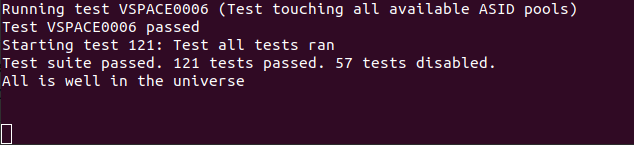
\includegraphics[width=\linewidth]{img/PrimaSimulazione.png}
  \caption{Primo avvio di seL4}
  \label{fig:PrimaSimulazione}
\end{figure}

\section{Programmazione con le API livello \textit{kernel} di seL4}
Una volta procurati tutti i prerequisiti necessari e appurato che seL4 può essere eseguito senza problemi, è finalmente possibile iniziare a prendere familiarità con il sistema, seguendo \textit{tutorial} forniti dalla \textit{seL4 Foundation} \cite{seL4Tutorial}. Tali \textit{tutorial} contengono programmi semicompleti, creati appositamente per sperimentare e far comprendere le funzionalità del sistema, in particolare con le API di seL4 \cite{sel4API}.\\
Come ormai già visto più volte sopra, si otterrà l'ambiente idoneo per eseguire i \textit{tutorial}, attraverso l'uso di \texttt{repo}:
\begin{lstlisting}[language=bash]
mkdir sel4-tutorials-manifest
cd sel4-tutorials-manifest
repo init -u https://github.com/seL4/sel4-tutorials-manifest
repo sync
\end{lstlisting}
Ogni \textit{tutorial} ha un suo \textit{repository} da importare nell'ambiente di lavoro nel quale, tra gli altri \textit{file} e cartelle, c'è (solitamente) un \texttt{main.c}, che sarà quello su cui andare ad apportare le modifiche per completare il \textit{tutorial} stesso.

\subsection{\textit{Capability}}
Come già detto nel capitolo precedente, una \textit{capability} è un \textit{token} unico, che dà accesso ad un'entità del sistema, un puntatore con dei diritti di accesso; in seL4 ci sono 3 tipi di \textit{capability}:
\begin{enumerate}
	\item \textit{capability} che controllano l'accesso ad entità del \textit{kernel}, come i \textit{thread control block} (TCB);
	\item \textit{capability} che controllano l'accesso a risorse astratte tipo gli \textit{interrupt};
	\item \textit{untyped capability} che sono responsabili della gestione della memoria.
\end{enumerate}

Tutte le \textit{capability} delle risorse del \textit{kernel} sono date dal processo \textit{root} all'inizializzazione del sistema, un po' come il processo \texttt{init} nei sistemi unix, che è padre di tutti i processi. Quando parliamo di \textit{capability} ci sono 3 termini fondamentali: CNode, CSlot e CSpace. Il primo di questi è l'abbreviazione di \textit{Capability-Node}, un oggetto che contiene delle \textit{capability}: si può pensarlo come un vettore (\textit{array}) di \textit{capability}. Ogni elemento dell'\textit{array} è chiamato CSlot (\textit{Capability-Slot}), il quale può avere due stati: \texttt{empty} o \texttt{full}. Ciò significa, rispettivamente, che il CNode ha una \textit{capability} nulla oppure una \textit{capability} ad una risorsa del \textit{kernel}. Per convenzione il primo CSlot, cioè quello situato alla posizione 0 del vettore, è nullo. Invece un CSpace (\textit{Capability-Space}) è il \textit{range} completo di \textit{capability} accessibile da un \textit{thread}, che può essere composto da uno o più CNode.

Per fare riferimento ad una \textit{capability} ed eseguire operazioni su di essa, è necessario fare un \texttt{address} (indirizzamento) della \textit{capability}. Ci sono due modi in seL4: tramite \textit{invocazione} o con \textit{indirizzamento diretto}.

Per quanto riguarda l'invocazione, ogni \textit{thread} ha uno speciale CNode installato nel suo TCB noto come \texttt{CSpace root}. Questo può essere nullo, ad esempio quando il \textit{thread} non è autorizzato a invocare nessuna \textit{capability}, o può avere una \textit{capability} ad un noto CNode. Quando si vuole fare un \textit{addressing} di una \textit{capability} attraverso invocazione, un CSlot viene indirizzato implicitamente, invocando il CSpace \textit{root} del \textit{thread} che sta facendo l'invocazione.

Per quanto riguarda il metodo dell'indirizzamento diretto, questo invece permette di specificare il CNode, piuttosto che utilizzare implicitamente il CSpace \textit{root}. Questo tipo di \textit{addressing}  è usato principalmente per costruire e manipolare i CSpace, potenzialmente il CSpace di un altro \textit{thread}.

L'esercizio proposto in questa sezione è un programma in linguaggio C con una serie di errori da risolvere, il primo tra questi è nel settaggio del numero di \textit{byte} del CNode:
\begin{lstlisting}[language=C++]
int main(int argc, char *argv[]) {

    /* parse the location of the seL4_BootInfo data structure from
    the environment variables set up by the default crt0.S */
    seL4_BootInfo *info = platsupport_get_bootinfo();

    size_t initial_cnode_object_size = BIT(info->initThreadCNodeSizeBits);
    printf("Initial CNode is %zu slots in size\n", initial_cnode_object_size);
    size_t initial_cnode_object_size_bytes = 0; // TODO
    printf("The CNode is %zu bytes in size\n", 	initial_cnode_object_size_bytes);
\end{lstlisting}

Chiaramente \texttt{initial\_cnode\_object\_size\_bytes} non può essere 0, il suo valore altresì dato sarà dato dal numero degli \textit{slot} del CNode moltiplicato per le dimensioni in \textit{bit} di ognuno di essi: \texttt{initial\_cnode\_object\_size * (1u << seL4\_SlotBits)}.

Eseguendo nuovamente il codice, questo darà l'errore \texttt{Attempted to invoke a null cap}. Ciò accade perché il codice cerca di impostare la priorità del TCB del \textit{thread}, invocando l'ultimo CSlot del CSpace, che però è vuoto:
\begin{lstlisting}[language=C++]
seL4_CPtr first_free_slot = info->empty.start;
seL4_Error error = seL4_CNode_Copy(seL4_CapInitThreadCNode, 
           first_free_slot, seL4_WordBits, seL4_CapInitThreadCNode,
           seL4_CapInitThreadTCB, seL4_WordBits, seL4_AllRights);
ZF_LOGF_IF(error, "Failed to copy cap!");
%seL4_CPtr last_slot = info->empty.end - 1;
// TODO

/* set the priority of the root task */
error = seL4_TCB_SetPriority(last_slot, last_slot, 10);
ZF_LOGF_IF(error, "Failed to set priority");
\end{lstlisting}

Per risolvere dunque il problema è necessario fare un'altra copia della \textit{capability} del TCB all'interno dell'ultimo slot del CNode: viene utilizzato \texttt{seL4\_CNode\_Copy}, che prende come parametri \texttt{destination root, slot, depth, source root, slot, depth} e \texttt{rights}, dove \texttt{depth} indica quanto bisogna attraversare il CNode per arrivare al CSlot e \texttt{rights} sono invece i diritti ereditati dalla nuova \textit{capability}; \texttt{first\_free\_slot} è lo \textit{slot} in cui è stata fatta una copia della \textit{capability} del TCB del \textit{thread} iniziale qualche riga di codice sopra:
\begin{lstlisting}[language=C++]
seL4_CNode_Copy(seL4_CapInitThreadCNode, last_slot, seL4_WordBits, seL4_CapInitThreadCNode, first_free_slot, seL4_WordBits, seL4_AllRights);
\end{lstlisting}

Rieseguendo il programma non viene più mostrato l'errore precedente, ma è comunque presente un altro errore \texttt{first\_free\_slot is not empty}. Questo avviene perché il codice cerca di spostare \texttt{first\_free\_slot} e \texttt{last\_slot} in se stesso; ciò non è possibile (perché è già presente una \textit{capability}, cioè se stessa) ed è in realtà un \textit{escamotage} per controllare se un CSlot è vuoto:
\begin{lstlisting}[language=C++]
// TODO 
         
// check first_free_slot is empty
error = seL4_CNode_Move(seL4_CapInitThreadCNode, first_free_slot,
                        seL4_WordBits, seL4_CapInitThreadCNode, 
                        first_free_slot, seL4_WordBits);
ZF_LOGF_IF(error != seL4_FailedLookup, "first_free_slot is not empty");

// check last_slot is empty
error = seL4_CNode_Move(seL4_CapInitThreadCNode, last_slot, seL4_WordBits,
                        seL4_CapInitThreadCNode, last_slot, seL4_WordBits);
ZF_LOGF_IF(error != seL4_FailedLookup, "last_slot is not empty");
\end{lstlisting}

Perciò per risolvere il problema bisogna eliminare le due \textit{capability}, questo può essere fatto eliminando le due copie delle \textit{capability} usando \texttt{seL4\_CNode\_Delete}, oppure con \texttt{seL4\_CNode\_Revoke} sulla \textit{capability} originale da cui sono state fatte le copie; quest'ultima API elimina tutte le \textit{capability} figlie di essa. Per fare più velocemente, si utilizzerà il secondo metodo, che richiede come parametri il CNode e la posizione dentro di esso in cui andare a recuperare la \textit{capability} (\texttt{CNode, index, depth}):
\begin{lstlisting}[language=C++]
seL4_CNode_Revoke(seL4_CapInitThreadCNode, seL4_CapInitThreadTCB, seL4_WordBits);
\end{lstlisting}

L'esercitazione si conclude con la sospensione del \textit{thread} corrente:
\begin{lstlisting}[language=C++]
seL4_TCB_Suspend(seL4_CapInitThreadTCB);
\end{lstlisting}
Il codice completo del \textit{tutorial} è riportato in \cite{capability}.

\subsection{Gestione della memoria}
Nella sezione precedente sono stati elencati i tipi di \textit{capability} presenti in seL4, al terzo posto nell'elenco si trovano le \textit{untyped capability}, il modo con il quale è possibile gestire la memoria fisica nel \textit{microkernel} seL4.

Ad eccezione di una piccola parte di memoria del \textit{kernel}, tutta la restante è gestita a livello utente. Le \textit{capability} di tutta la memoria fisica disponibile vengono passate al processo \textit{root} come \textit{capability} alla \textit{untyped memory}, che altro non è che un blocco contiguo di memoria fisica con una dimensione ben specifica. Per riassumere, in seL4 si avranno quindi le \textit{untyped capability} che sono \textit{capability} per la \textit{untyped memory}. Inoltre le \textit{untyped capability} possono essere riscritte in oggetti del \textit{kernel} insieme alla \textit{capability}, oppure in ulteriori \textit{untyped capability} più piccole.

Le \textit{untyped capability} hanno anche un \textit{flag} booleano \textit{device}, che indica se la memoria è scrivibile dal \textit{kernel} oppure no: può essere in un'area non accessibile dal \textit{kernel} o riservata ad altri dispositivi.

In seL4 esiste un unico modo per invocare una \textit{untyped capability}, cioè attraverso l'utilizzo dell'API \texttt{seL4\_Untyped\_Retype}, che serve per creare una nuova \textit{capability} da una \textit{untyped capability}. Nello specifico, questo \textit{retype} darà accesso ad un sottoinsieme della memoria della \textit{capability} di origine, che può essere una \textit{untyped capability} più piccola o può puntare ad un nuovo oggetto con un tipo specifico:
\begin{lstlisting}[language=C++]
seL4_Untyped_Retype(parent_untyped, // the untyped capability to retype
                    seL4_UntypedObject, // type
                    untyped_size_bits,  //size
                    seL4_CapInitThreadCNode, // root
                    0, // node_index
                    0, // node_depth
                    child_untyped, // node_offset
                    1); // num_caps
\end{lstlisting}

Le \textit{untyped capability} sono riscritte in maniera incrementale seguendo una politica \textit{greedy}, a partire dall'\textit{untyped} invocato. Ogni \textit{untyped capability} mantiene un singolo \textit{watermark}, con gli indirizzi prima di esso non disponibili e quelli successivi liberi. La memoria non può essere liberata fino a che tutti i figli non vengono revocati, laddove i figli non sono altro che le nuove \textit{capability}, che vengono create da una \textit{untyped capability}.

Come per la sezione precedente anche qui è presente un \textit{repository} da scaricare con all'interno un file\texttt{ main.c}, che una volta compilato e avviato, stampa a video una lista di tutte le \textit{untyped capability} fornite dal processo \textit{root} all'avvio e segnala un errore \texttt{Untyped Retype: Requested UntypedItem size too small}. Ciò succede perché il programma sta tentando di creare una \textit{untyped} di dimensione 0:
\begin{lstlisting}[language=C++]
int main(int argc, char *argv[]) {
    /* parse the location of the seL4_BootInfo data structure from
    the environment variables set up by the default crt0.S */
    seL4_BootInfo *info = platsupport_get_bootinfo();


    printf("    CSlot   \tPaddr           \tSize\tType\n");
    for (seL4_CPtr slot = info->untyped.start; slot != info->untyped.end;
    slot++) {
        seL4_UntypedDesc *desc = 
                 &info->untypedList[slot - info->untyped.start];
        printf("%8p\t%16p\t2^%d\t%s\n", (void *) slot, 
              (void *) desc->paddr, desc->sizeBits, 
              desc->isDevice ? "device untyped" : "untyped");
    }
    seL4_Error error;

    // list of general seL4 objects
    seL4_Word objects[] = {seL4_TCBObject, seL4_EndpointObject,
                           seL4_NotificationObject};
    // list of general seL4 object size_bits
    seL4_Word sizes[] = {seL4_TCBBits, seL4_EndpointBits,
                         seL4_NotificationBits};
    
    // TODO
    seL4_Word untyped_size_bits = 0; //ERRORE GENERATO QUI
    seL4_CPtr parent_untyped = 0;
    seL4_CPtr child_untyped = info->empty.start;

    // First, find an untyped big enough to fit all of our objects
    for (int i = 0; i < (info->untyped.end - info->untyped.start); i++) {
        if (info->untypedList[i].sizeBits >= 
                   untyped_size_bits && !info->untypedList[i].isDevice) {
                   
            parent_untyped = info->untyped.start + i;
            break;
        }
    }
\end{lstlisting}

Per risolvere questo problema si deve assegnare una dimensione consona alla variabile \texttt{untyped\_size\_bits}. Dato che si deve creare uno spazio per tutti gli elementi di \texttt{objects[]} e considerato che la somma di \texttt{seL4\_EndpointBits} e \texttt{seL4\_NotificationBits} è inferiore a \texttt{seL4\_TCBBits}, si può attribuire alla variabile il valore \texttt{seL4\_TCBBits + 1}. Il +1 fa raddoppiare il numero di \textit{byte}, visto che lo spazio assegnato sarà $ 2^{seL4\_TCBBits + 1} $ \textit{bit}, i quali sono sufficienti per contenere tutti e tre gli elementi.

Eseguendo di nuovo il programma, questo procederà fino a che non segnalerà un ulteriore errore \texttt{Failed to set priority}:
\begin{lstlisting}[language=C++]
// create an untyped big enough to retype all of the above objects from
error = seL4_Untyped_Retype(parent_untyped, seL4_UntypedObject, untyped_size_bits, seL4_CapInitThreadCNode, 0, 0, child_untyped, 1);
ZF_LOGF_IF(error != seL4_NoError, "Failed to retype");

// use the slot after child_untyped for the new TCB cap:
seL4_CPtr child_tcb = child_untyped + 1;
// TODO

// try to set the TCB priority
error = seL4_TCB_SetPriority(child_tcb, seL4_CapInitThreadTCB, 10);
ZF_LOGF_IF(error != seL4_NoError, "Failed to set priority");
\end{lstlisting}

L'errore viene generato perché \texttt{child\_tcb} è un CSlot vuoto. Per risolvere è sufficiente assegnare al CSlot una \textit{capability}, creando un \textit{TCB object} da \texttt{child\_untyped}:
\begin{lstlisting}[language=C++]
seL4_Untyped_Retype(child_untyped, seL4_TCBObject, 0, seL4_CapInitThreadCNode, 0, 0, child_tcb, 1);
\end{lstlisting}

Con questa linea di codice il problema è sì risolto, ma l'esecuzione viene bloccata da un altro errore \texttt{Endpoint cap is null cap}:
\begin{lstlisting}[language=C++]
// use the slot after child_tcb for the new endpoint cap:
seL4_CPtr child_ep = child_tcb + 1;
// TODO

// identify the type of child_ep
uint32_t cap_id = seL4_DebugCapIdentify(child_ep);
ZF_LOGF_IF(cap_id == 0, "Endpoint cap is null cap");
\end{lstlisting}

Tale errore è molto simile al precedente: si sta cercando di identificare un \textit{endpoint} nullo. Quindi per risolvere il problema è va creato un \textit{endpoint object} sempre da \texttt{child\_untyped} e mettere la \textit{capability} nel CSlot \texttt{child\_ep}:
\begin{lstlisting}[language=C++]
seL4_Untyped_Retype(child_untyped, seL4_EndpointObject, 0, seL4_CapInitThreadCNode, 0, 0, child_ep, 1);
\end{lstlisting}

Alla fine il programma tenta di allocare tutto il \texttt{child\_untyped} come \textit{endpoint}, ma fallisce perché tutto lo spazio è stato esaurito dalle allocazioni fatte precedentemente. La soluzione al problema è eseguire una \texttt{seL4\_CNode\_Revoke} (vista sopra) su di esso, in modo che tutto le spazio venga liberato e così facendo il programma termina con successo:
\begin{lstlisting}[language=C++]
// revoke the child untyped
error = seL4_CNode_Revoke(seL4_CapInitThreadCNode, child_untyped, seL4_WordBits);

// allocate the whole child_untyped as endpoints
// Remember the sizes are exponents, so this computes 2^untyped_size_bits / 2^seL4_EndpointBits:
seL4_Word num_eps = BIT(untyped_size_bits - seL4_EndpointBits);
error = seL4_Untyped_Retype(child_untyped, seL4_EndpointObject, 0, seL4_CapInitThreadCNode, 0, 0, child_tcb, num_eps);
ZF_LOGF_IF(error != seL4_NoError, "Failed to create endpoints.");

printf("Success\n");
\end{lstlisting}
Il codice completo del \textit{tutorial} è riportato in \cite{untyped}.

\subsection{\textit{Virtual memory management}}
SeL4 non fornisce strumenti per la gestione della memoria virtuale al di là delle primitive per la gestione dell'\textit{hardware}; quindi il servizio di \textit{mapping} della memoria e lo \textit{swapping} devono essere gestiti a livello utente, che ha tutta la libertà di procedere in base alle esigenze del sistema. SeL4 mette dunque a disposizione degli oggetti appositi chiamati \textit{VSpace} (\textit{virtual address space}), simili ai CSpace, che sono composti da oggetti forniti dal \textit{kernel}, che variano in base all'architettura \textit{hardware} (x86\_64, RISC-V, ARM).

Per mappare le pagine sono necessari degli \textit{intermediate hardware virtual memory objects}: in pratica si deve creare una struttura intermedia, che varia in base all'architettura. Ad esempio nei sistemi x86\_64 per mappare una pagina sono necessari questi 3 oggetti: \texttt{seL4\_PDPT, seL4\_PageDirector,} e \texttt{seL4\_PageTable}. 

Le API di seL4 forniscono varie funzioni per la mappatura della memoria in base all'architettura in cui sta girando seL4. Tutte le funzioni di \textit{mapping} prendono 3 argomenti principali:
\begin{itemize}
	\item il VSpace in cui mappare l'oggetto;
	\item l'indirizzo virtuale su cui mappare l'oggetto;
	\item gli attributi della memoria virtuale che dipendono dall'architettura.
\end{itemize}
Un esempio di mappatura di un oggetto \texttt{seL4\_PDPT} ad un certo indirizzo \texttt{TEST\_VADDR} è:
\begin{lstlisting}[language=C++]
seL4_X86_PDPT_Map(pdpt, seL4_CapInitThreadVSpace, TEST_VADDR, seL4_X86_Default_VMAttributes);
\end{lstlisting}

Una volta che le strutture di paginazione intermedie sono state mappate in un certo \textit{range} di indirizzi virtuali, i \textit{frame} fisici possono essere mappati in quel \textit{range} attraverso l'invocazione del \textit{frame capability}.\\
Ecco un esempio di mappatura di un \textit{frame}:
\begin{lstlisting}[language=C++]
seL4_X86_Page_Map(frame, seL4_CapInitThreadVSpace, TEST_VADDR, seL4_CanRead, seL4_X86_Default_VMAttributes);
\end{lstlisting}

Come si può notare, questo metodo prende un argomento in più, perché per mappare i \textit{frame} vengono richiesti anche i diritti che determineranno il tipo di mappatura (nell'esempio sopra diritti di sola lettura).

Il \textit{tutorial} di questa sezione fornisce un programma che all'avvio presenta l'errore \texttt{Missing intermediate paging structure at level 30}:
\begin{lstlisting}[language=C++]
int main(int argc, char *argv[]) {
    /* parse the location of the seL4_BootInfo data structure from
    the environment variables set up by the default crt0.S */
    seL4_BootInfo *info = platsupport_get_bootinfo();
    seL4_Error error;
    seL4_CPtr frame = alloc_object(info, seL4_X86_4K, 0);
    seL4_CPtr pdpt = alloc_object(info, seL4_X86_PDPTObject, 0);
    seL4_CPtr pd = alloc_object(info, seL4_X86_PageDirectoryObject, 0);
    seL4_CPtr pt = alloc_object(info, seL4_X86_PageTableObject, 0);

	// TODO
	
	// TODO

    /* map a PDPT at TEST_VADDR */
    error = seL4_X86_PDPT_Map(pdpt, seL4_CapInitThreadVSpace, TEST_VADDR, seL4_X86_Default_VMAttributes);

    /* map a read-only page at TEST_VADDR */
    error = seL4_X86_Page_Map(frame, seL4_CapInitThreadVSpace, TEST_VADDR, seL4_CanRead, seL4_X86_Default_VMAttributes);
    if (error == seL4_FailedLookup) {
        printf("Missing intermediate paging structure at level %lu\n", seL4_MappingFailedLookupLevel());
    }
    ZF_LOGF_IF(error != seL4_NoError, "Failed to map page");
\end{lstlisting}

L'errore è dovuto al fatto che per mappare una pagina, tutte le strutture di paginazione intermedie devono essere mappate; il valore \texttt{30} equivale alla costante \texttt{SEL4\_MAPPING\_LOOKUP\_NO\_PD}, il che indica che è necessario mappare un oggetto \textit{page directory}, che può essere fatto con l'apposito metodo \texttt{seL4\_X86\_PageDirectory\_Map}:
\begin{lstlisting}[language=C++]
seL4_X86_PageDirectory_Map(pd, seL4_CapInitThreadVSpace, TEST_VADDR, seL4_X86_Default_VMAttributes);
\end{lstlisting}

Ricompilando ed eseguendo il codice appare un errore simile al precedente \texttt{Missing intermediate paging structure at level 21}, dove il valore \texttt{21} questa volta, indica la costante \texttt{SEL4\_MAPPING\_LOOKUP\_NO\_PT} che suggerisce di mappare un oggetto di tipo \textit{page table}:
\begin{lstlisting}[language=C++]
seL4_X86_PageTable_Map(pt, seL4_CapInitThreadVSpace, TEST_VADDR, seL4_X86_Default_VMAttributes);
\end{lstlisting}

Adesso il codice procede mappando la pagina; successivamente però (come si può leggere nel codice sotto riportato) avviene un tentativo di scrittura sulla pagina, che genera un errore perché la pagina era stata mappata in sola lettura \texttt{seL4\_CanRead}. L'errore può dunque essere evitato facendo una rimappatura della pagina, questa volta in lettura e scrittura:
\begin{lstlisting}[language=C++]
seL4_X86_Page_Map(frame, seL4_CapInitThreadVSpace, TEST_VADDR, seL4_ReadWrite, seL4_X86_Default_VMAttributes);
\end{lstlisting}

Il \textit{mapping} delle pagine può anche essere disfatto utilizzando \texttt{unmap} sulla pagina o su qualsiasi struttura intermedia di paginazione; in alternativa può essere eseguito eliminando la \textit{capability} finale di qualsiasi struttura di paginazione.\\
Il codice completo del \textit{tutorial} è riportato in \cite{mapping}.

\subsection{\textit{Thread}}
SeL4, per rappresentare l'esecuzione di un processo e gestirne i tempi di esecuzione, fornisce i \textit{thread}. Essi sono realizzati attraverso \textit{thread control block object} (TCBs), uno per ogni \textit{thread} del kernel.

Come noto, in un SO è lo \textit{scheduler} a decidere quale processo e per quanto tempo può utilizzare la CPU. In seL4, come già visto nel capitolo precedente, la politica di \textit{scheduling} è un'integrazione di \textit{round-robin} e \textit{scheduling a priorità}: lo \textit{scheduler} sceglie i \textit{thread} con maggiore priorità che sono pronti e se ce ne sono con la stessa priorità, questi saranno scelti in ordine FIFO, seconda la politica \textit{round-robin}. La priorità è determinata da un \textit{range} che va da 0 (\texttt{seL4\_MinPrio}) a 255 (\texttt{seL4\_MaxPrio}). Oltre alla priorità, un TCBs contiene anche un \textit{maximum control priority} (MCP), che serve per controllare che un processo non modifichi la priorità di un altro processo (o di se stesso), impostandola più alta della sua. Quindi un processo che vuole modificare una priorità deve fornire la sua \textit{capability} (di \textit{thread}), in modo da determinare se è autorizzato a impostare quella priorità.

L'esercizio per questa sezione, se fatto partire senza nessuna modifica, inizialmente mostrerà a video una tabella di tutti i TCB (questo è ottenuto tramite una chiamata di sistema di debug \texttt{seL4\_DebugDumpScheduler()}) e successivamente lancia un errore \texttt{Failed to retype thread: 2} come in Figura~\ref{fig:TutorialThreads}:\\
\begin{figure}[h]
  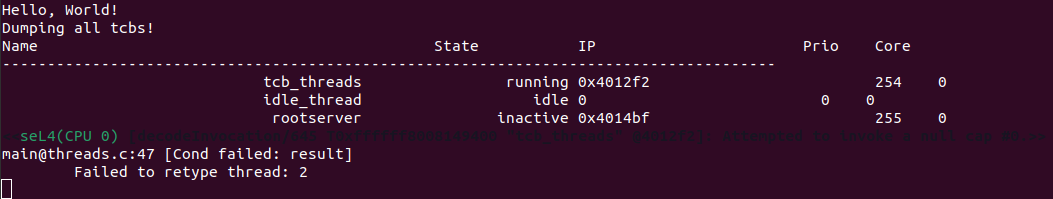
\includegraphics[width=\linewidth]{img/Threads.png}
  \caption{lista TCB}
  \label{fig:TutorialThreads}
\end{figure}

Questo errore avviene perché c'è un'errata invocazione del metodo: \texttt{seL4\_Untyped\_Retype()}.
\begin{lstlisting}[language=C++]
// the root CNode of the current thread
extern seL4_CPtr root_cnode;
// VSpace of the current thread
extern seL4_CPtr root_vspace;
// TCB of the current thread
extern seL4_CPtr root_tcb;
// Untyped object large enough to create a new TCB object

extern seL4_CPtr tcb_untyped;
extern seL4_CPtr buf2_frame_cap;
extern const char buf2_frame[4096];

// Empty slot for the new TCB object
extern seL4_CPtr tcb_cap_slot;
// Symbol for the IPC buffer mapping in the VSpace, and capability to the mapping
extern seL4_CPtr tcb_ipc_frame;
extern const char thread_ipc_buff_sym[4096];
// Symbol for the top of a 16 * 4KiB stack mapping, and capability to the mapping
extern const char tcb_stack_base[65536];
static const uintptr_t tcb_stack_top = (const uintptr_t)&tcb_stack_base + sizeof(tcb_stack_base);

int new_thread(void *arg1, void *arg2, void *arg3) {
    printf("Hello2: arg1 %p, arg2 %p, arg3 %p\n", arg1, arg2, arg3);
    void (*func)(int) = arg1;
    func(*(int *)arg2);
    while(1);
}

int main(int c, char* arbv[]) {

    printf("Hello, World!\n");

    seL4_DebugDumpScheduler();
	// TODO
    seL4_Error result = seL4_Untyped_Retype(seL4_CapNull, seL4_TCBObject, seL4_TCBBits, seL4_CapNull, 0, 0, seL4_CapNull, 1);
    ZF_LOGF_IF(result, "Failed to retype thread: %d", result);
    seL4_DebugDumpScheduler();
\end{lstlisting}

Come si può evincere, al metodo viene passato un oggetto \texttt{seL4\_CapNull} come oggetto da riscrivere, che ovviamente genera l'errore. Dunque un modo corretto per ovviare a questo errore è utilizzare gli oggetti creati nelle variabili globali del codice:
\begin{lstlisting}[language=C++]
seL4_Error result = seL4_Untyped_Retype(tcb_untyped, seL4_TCBObject, seL4_TCBBits, root_cnode, 0, 0, tcb_cap_slot, 1);
\end{lstlisting}

Rieseguendo il codice, si noterà che l'errore è risolto e tra la lista dei TCB adesso è presente anche quello appena creato. Dopo aver risolto questo problema, si presenta un errore \texttt{Failed to configure thread: 2}, in quanto la configurazione del TCB viene fatta tutta su valori nulli:
\begin{lstlisting}[language=C++]
result = seL4_TCB_Configure(seL4_CapNull, seL4_CapNull, 0, seL4_CapNull, 0, 0, (seL4_Word) NULL, seL4_CapNull);
ZF_LOGF_IF(result, "Failed to configure thread: %d", result);
\end{lstlisting}

Il metodo \texttt{seL4\_TCB\_Configure} prende come parametri:
\begin{lstlisting}[language=C++]
seL4_TCB_Configure(tcb, // tcb su cui operare
					cspace_root, // nuovo CSpace root
					cspace_root_data, // opzionale: setta il nuovo CNode
					vspace_root, // nuovo VSpace root
					vspace_root_data, // non ha effetto su x86 e ARM
					buffer, // locazione dell'IPC buffer
					bufferFrame); // IPC buffer
\end{lstlisting} 

Si può quindi procedere alla corretta configurazione del TCB in modo tale da avere lo stesso CSpace e VSpace del \textit{thread} corrente:
\begin{lstlisting}[language=C++]
result = seL4_TCB_Configure(tcb_cap_slot, seL4_CapNull, root_cnode, 0, root_vspace, 0, (seL4_Word) thread_ipc_buff_sym, tcb_ipc_frame);
\end{lstlisting}

Adesso l'errore che si presenta sarà un altro
\texttt{Failed to set the priority for the new TCB object}: questo accade perché la priorità data al \textit{thread} ha valore 0:
\begin{lstlisting}[language=C++]
result = seL4_TCB_SetPriority(tcb_cap_slot, seL4_CapNull, 0);
ZF_LOGF_IF(result, "Failed to set the priority for the new TCB object.\n");
seL4_DebugDumpScheduler();
\end{lstlisting}

Il \textit{thread} corrente ha un MCP di 254 quindi è possibile assegnare questo valore come priorità, ma è necessario anche cambiare il valore \texttt{seL4\_CapNull} e sostituirlo con il TCB del \textit{thread} corrente \texttt{root\_tcb}, dopodiché impostare in maniera adeguata i registri iniziali, in particolare il \textit{program counter} e lo \textit{stack pointer}. Ciò è possibile grazie alle \textit{utility} contenute in \texttt{libsel4utils}:
\begin{lstlisting}[language=C++]
seL4_UserContext regs = {0};
int error = seL4_TCB_ReadRegisters(tcb_cap_slot, 0, 0, sizeof(regs)/sizeof(seL4_Word), &regs);
ZF_LOGF_IFERR(error, "Failed to read the new thread's register set.\n");

// TODO
sel4utils_set_instruction_pointer(&regs, (seL4_Word)new_thread);
// TODO
sel4utils_set_stack_pointer(&regs, tcb_stack_top);
// TODO
error = seL4_TCB_WriteRegisters(tcb_cap_slot, 0, 0, sizeof(regs)/sizeof(seL4_Word), &regs);
ZF_LOGF_IFERR(error, "Failed to write the new thread's register set.\n"
                  "\tDid you write the correct number of registers? See arg4.\n");
seL4_DebugDumpScheduler();
\end{lstlisting}

A questo punto si farà partire partire il \textit{thread}, ma con un piccolo aggiustamento nel codice:
\begin{lstlisting}[language=C++]
//resume the new thread
error = seL4_TCB_Resume(seL4_CapNull);
ZF_LOGF_IFERR(error, "Failed to start new thread.\n");
while(1);
return 0;
}
\end{lstlisting}

Chiaramente il \texttt{seL4\_TCB\_Resume} va fatto sul nostro \texttt{tcb\_cap\_slot} e non su \texttt{seL4\_CapNull}. Ora il nuovo \textit{thread} viene eseguito e mostra a video\\
\texttt{Hello2: arg1 0, arg2 0, arg3 0}.

I valori passati al nuovo \textit{thread} sono tutti 0. Se volessimo però passare al \textit{thread} valori differenti, si potrebbe utilizzare la funzione \texttt{sel4utils\_arch\_init\_local\_context}, con le dovute modifiche al codice:
\begin{lstlisting}[language=C++]
UNUSED seL4_UserContext regs = {0};
int error = seL4_TCB_ReadRegisters(tcb_cap_slot, 0, 0, sizeof(regs)/sizeof(seL4_Word), &regs);
ZF_LOGF_IFERR(error, "Failed to read the new thread's register set.\n"
              "\tDid you write the correct number of registers? See arg4.\n");

sel4utils_arch_init_local_context((void*)new_thread,
                                  (void *)1, (void *)2, (void *)3,
                                  (void *)tcb_stack_top, &regs);
error = seL4_TCB_WriteRegisters(tcb_cap_slot, 0, 0, sizeof(regs)/sizeof(seL4_Word), &regs);
ZF_LOGF_IFERR(error, "Failed to write the new thread's register set.\n"
              "\tDid you write the correct number of registers? See arg4.\n");
\end{lstlisting}
Il codice completo del \textit{tutorial} è riportato in \cite{threads}.

\subsection{IPC}
\textit{InterProcess Communication} è il meccanismo che utilizza il \textit{microkernel} per sincronizzare lo scambio di  piccole quantità di dati e \textit{capability} tra i processi. In seL4 l'IPC è facilitato dal fatto che gli oggetti del \textit{kernel} sono di piccole dimensioni, noti come \textit{endpoint} e fungono da porte per la comunicazione; quindi per mandare e ricevere messaggi IPC bisogna procedere attraverso invocazioni sugli \textit{endpoint}.

I \textit{thread} possono mandare messaggi sugli \textit{endpoint} con la \textit{system call} \texttt{seL4\_Send} che è bloccante, mentre possono usare \texttt{seL4\_Recv} per ricevere messaggi.

\texttt{seL4\_Call} invece è una chiamata di sistema che combina le due precedenti con una differenza: nella fase di ricezione il \textit{thread} che usa questa funzione è bloccato su una \textit{one-time capability} chiamata \textit{reply capability} e non sull'\textit{endpoint} stesso, come avverrebbe normalmente con la \texttt{seL4\_Recv}. La \textit{replay capability} è contenuta nel TCB del ricevente.

La \textit{system call} \texttt{seL4\_Reply} invoca la \textit{reply capability}, la quale manderà un IPC che farà risvegliare il processo bloccato. \texttt{seL4\_ReplyRecv} fa lo stesso, ma invia la risposta e blocca l'\textit{endpoint} fornito in una chiamata di sistema combinata.

Ogni \textit{thread} ha un \textit{buffer} che contiene il \textit{payload} del messaggio IPC composto da dati e \textit{capability}. Il mittente del messaggio specifica la lunghezza e il \textit{kernel} copia questa quantità tra il mittente e il destinatario dell'\textit{IPC buffer}. Quest'ultimo contiene un'area limitata di registri di messaggio (\textit{message registers}, abbreviato MR), che sono utilizzati per trasmettere dati sull'IPC. Ogni registro ha dimensione di una parola (\textit{word}) (dimensione relativa alla macchina) e la lunghezza massima di un messaggio è contenuta nella costante \texttt{seL4\_MsgMaxLength}. Per caricare un messaggio all'interno del \textit{buffer} è possibile utilizzare \texttt{seL4\_SetMR}, mentre per estrarlo \texttt{seL4\_GetMR}; la quantità di parole che possono entrare in un registro è disponibile nella costante \texttt{seL4\_FastMessageRegisters}.

Insieme al messaggio, il \textit{kernel} consegna il \textit{badge} dell'\textit{endpoint capability}, sul quale il mittente ha fatto l'invocazione per mandare il messaggio. È possibile assegnare un \textit{badge} all'\textit{endpoint}, utilizzando \texttt{seL4\_CNode\_Mint} oppure \texttt{seL4\_CNode\_Mutate}; una volta che è stato messo il \textit{badge} sull'\textit{endpoint}, questo viene trasferito a tutti i destinatari che ricevono un messaggio su quell'\textit{endpoint}.

SeL4, per codificare la descrizione di un messaggio IPC, usa la struttura dati \texttt{seL4\_MessageInfo\_t},la quale ha la dimensione di una parola ed è composta dai seguenti campi: 
\begin{itemize}
	\item[-] \texttt{length} la quantità di dati nel messaggio;
	\item[-] \texttt{extraCaps} numero di \textit{capability} nel messaggio;
	\item[-] \texttt{capsUnwrapped} marca le \textit{capability unwrapped} del \textit{kernel};
	\item[-] \texttt{label} dati che verranno trasferiti che non sono stati modificati dal \textit{kernel}.
\end{itemize}

Come già accennato, insieme ai dati, attraverso l'IPC, è possibile scambiare anche \textit{capability}. In gergo questo viene chiamato \textit{cap transfer}:
\begin{lstlisting}[language=C++]
//Invio di una capability via IPC
seL4_MessageInfo info = seL4_MessageInfo_new(0, 0, 1, 0);
seL4_SetCap(0, free_slot);
seL4_Call(endpoint, info);

//Ricezione di una capability
seL4_SetCapReceivePath(cnode, badged_endpoint, seL4_WordBits);
seL4_Recv(endpoint, &sender);
\end{lstlisting}

Il numero di \textit{capability} trasferite è codificato nella struttura dati \texttt{seL4\_MessageInfo\_t} come \texttt{extraCaps}.
Inoltre seL4 può fare la cosiddetta \textit{unwrap} (scartare) delle \textit{capability} sull'IPC: se l'n-esima \textit{capability} nel messaggio si riferisce all'\textit{endpoint} attraverso il quale il messaggio viene inviato, la \textit{capability} viene \textit{unwrapped}: il suo badge viene inserito nell'n-esima posizione dell'IPC \textit{buffer} del destinatario (\texttt{caps\_or\_badges}) e il \textit{kernel} imposta l'n-esimo \textit{bit} nel campo \texttt{capsUnwrapped} del \texttt{seL4\_MessageInfo\_t}.

L'unico modo che hanno i processi per comunicare, nei sistemi basati su \textit{microkernel}, è attraverso l'utilizzo dell'IPC. Essendo tutti i servizi a livello utente si può intuire che di questa funzionalità ne verrà fatto un utilizzo massiccio. Quindi è necessario che sia realizzata al meglio e che magari si prevedano scorciatoie per renderla ancora più efficiente, in quanto da essa dipendono le prestazioni dell'intero sistema.

Per soddisfare questa esigenza è stato introdotto il \textit{fastpath}, cioè un cammino nel \textit{kernel} altamente ottimizzato, che garantisce velocità nell'IPC. Per potersi definire tale deve soddisfare cinque condizioni:
\begin{itemize}
	\item devono essere usate le \textit{system call} \texttt{seL4\_Call} o \texttt{seL4\_ReplyRecv};
	\item i dati del messaggio devono entrare nel registro \texttt{seL4\_FastMessageRegisters};
	\item i processi devono avere spazi di indirizzi validi;
	\item non dovrebbero essere trasferite \textit{capability};
	\item nessun altro \textit{thread} nello \textit{scheduler}, con priorità superiore a quello sbloccato dall'IPC, può essere in esecuzione.
\end{itemize}

In questa sezione l'esercizio è un po' diverso. Non c'è un unico \textit{file main} in cui è contenuto tutto il codice, ma c'è un \texttt{server.c} e due \textit{client} \texttt{client\_1.c} e \texttt{client\_2.c}, i quali manderanno dei messaggi al \textit{server}, che farà da \textit{echo}; tutti i processi hanno accesso ad un unico \textit{endpoint capability}, che fornisce accesso allo stesso \textit{endpoint object}. Al primo avvio si ha questo \textit{output}:
\begin{figure}[H]
  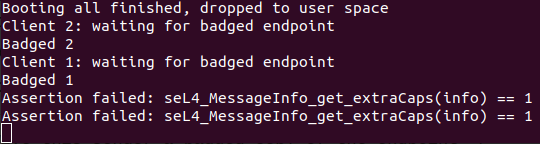
\includegraphics[scale=0.7]{img/PrimoAvvioIPC2.png}%width=\linewidth
  \centering
  \label{fig:PrimoAvvio}
\end{figure}

Gli errori sono dovuti al fatto che entrambi i \textit{client} si mettono in attesa, sull'\textit{endpoint} fornito, di un \textit{badged endpoint} tramite \textit{cap tranfer}, che però il \textit{server} non invierà, in quanto esso risponde solo ai messaggi dei \textit{client}:
\begin{lstlisting}[language=C++]
// cslot containing IPC endpoint capability
extern seL4_CPtr endpoint;
// cslot containing a capability to the cnode of the server
extern seL4_CPtr cnode;
// empty cslot
extern seL4_CPtr free_slot;

int main(int c, char *argv[]) {

	seL4_Word sender;
    seL4_MessageInfo_t info = seL4_Recv(endpoint, &sender);
    while (1) {
	    seL4_Error error;
        if (sender == 0) {

             /* No badge! give this sender a badged copy of the endpoint */
             seL4_Word badge = seL4_GetMR(0);
             seL4_Error error = seL4_CNode_Mint(cnode, free_slot,
                              seL4_WordBits, cnode, endpoint,
                              seL4_WordBits, seL4_AllRights, badge);
             printf("Badged %lu\n", badge);

             // TODO
             
             /* reply to the sender and wait for the next message */
             seL4_Reply(info);

             /* now delete the transferred cap */
             error = seL4_CNode_Delete(cnode, free_slot, seL4_WordBits);
             assert(error == seL4_NoError);

             /* wait for the next message */
             info = seL4_Recv(endpoint, &sender);
\end{lstlisting}

Dunque, per risolvere questo problema si imposterà il \textit{cap transfer} in modo tale che i \textit{client} ricevano il \textit{badged endpoint}:
\begin{lstlisting}[language=C++]
info = seL4_MessageInfo_new(0, 0, 1, 0);
seL4_SetCap(0, free_slot);
\end{lstlisting}

Compilando e riavviando il programma sembra che non ci siano problemi tranne per il fatto che il sistema si blocca, come si vede nella figura sottostante:
\begin{figure}[H]
  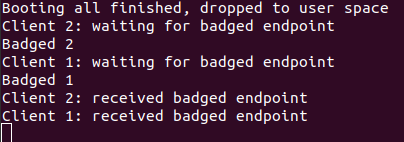
\includegraphics[scale=0.7]{img/DopoBadgeIPC.png}%width=\linewidth
  \centering
  \label{fig:AvvioDopoBadge}
\end{figure}

Ciò succede perché al \textit{server} manca l'implementazione della sua funzione di \textit{echo} dei messaggi che gli vengono inviati; tale funzione può essere fatta scorrendo e stampando a video il contenuto dei \textit{message register}.\\
I \texttt{client\_1} manda le stringhe {"quick", "fox", "over" e "lazy"}, mentre il \texttt{client\_2} le stringhe {"the", "brown", "jumps", "the" e "dog"}:
\begin{lstlisting}[language=C++]
for (int i = 0; i < seL4_MessageInfo_get_length(info); i++) {
printf("%c", (char) seL4_GetMR(i));
}
printf("\n");
\end{lstlisting}

A questo punto però si vedrà stampata a video sempre la stessa parola \texttt{the} in \textit{loop} perché il server non manda un \textit{feedback} di risposta al \textit{client} e di conseguenza continua a stampare l'ultima parola ricevuta:
\begin{lstlisting}[language=C++]
for (int i = 0; i < seL4_MessageInfo_get_length(info); i++) {
	printf("%c", (char) seL4_GetMR(i));
}
printf("\n");

// reply to the client and wait for the next message
info = seL4_ReplyRecv(endpoint, info , &sender);
\end{lstlisting}

Rieseguendo, (l'\textit{output} sarà la stampa a video prima di tutte le parole inviate dal \texttt{client\_2}, seguite da quelle del \texttt{client\_1}) si può modificare il codice in modo tale da alternare le stampe dei due \textit{client}, utilizzando \texttt{seL4\_CNode\_SaveCaller} e \texttt{free\_slot} per salvare le risposte:
\begin{lstlisting}[language=C++]
for (int i = 0; i < seL4_MessageInfo_get_length(info); i++) {
printf("%c", (char) seL4_GetMR(i));
}
printf("\n");

error = seL4_CNode_SaveCaller(cnode, free_slot, seL4_WordBits);
assert(error == 0);
info = seL4_Recv(endpoint, &sender);
for (int i = 0; i < seL4_MessageInfo_get_length(info); i++) {
   printf("%c", (char) seL4_GetMR(i));
}
printf("\n");
seL4_Send(free_slot, seL4_MessageInfo_new(0, 0, 0, 0));

// reply to the client and wait for the next message
info = seL4_ReplyRecv(endpoint, info, &sender);
\end{lstlisting}

Una volta eseguite tutte le correzioni, l'\textit{output} finale sarà il seguente:
\begin{lstlisting}[language=bash]
Client 2: received badged endpoint
the
Client 1: received badged endpoint
quick
fox
brown
jumps
over
lazy
the
dog
\end{lstlisting}
Il codice completo del \texttt{server} è riportato in \cite{IPCserver}.\\
Il codice completo del \texttt{client\_1} è riportato in \cite{IPCclient1}.\\
Il codice completo del \texttt{client\_2} è riportato in \cite{IPCclient2}.
\chapter{Conclusioni}
Giunti alla fase conclusiva della mia tesi, in cui è stato trattato in modo completo l'argomento seL4, ed essendo ormai chiaro cosa sia un sistema operativo, credo sia opportuno proporre alcune osservazioni.

Partendo dal presupposto che verosimilmente le persone a conoscenza dell'esistenza di seL4 siano molto poche, dato che è evidente che non sia tanto noto quanto i sistemi operativi Windows, Mac o Linux e che, come dimostrato nei capitoli precedenti del mio elaborato, si tratti di un sistema efficiente e sicuro, penso che sia stato inevitabile, durante la lettura, domandarsi il motivo per cui si sia sentito nominare questo \textit{microkernel} per la prima volta.

Analizzando diversi elementi, si può affermare che, essendo seL4 un \textit{microkernel}, i servizi che può offrire sono davvero pochi; pensare di realizzare un sistema operativo che ricalchi i tre sopra menzionati, altamente \textit{user-friendly}, diffusi su scala globale ed utilizzabili nella maggior parte delle situazioni, risulterebbe davvero complesso, considerato l'elevato numero di elementi da sviluppare partendo da zero. Altro aspetto certamente non secondario è la sicurezza: per la distribuzione di massa non è necessario avere un livello di protezione così elevato; quando si tratta di salvaguardia dei dati, non esiste un vero e proprio limite, specialmente oggi, in un contesto globale in cui "i dati sono il nuovo petrolio"\footnote{Clive Humby, 2006}, ma è assolutamente necessaria una valutazione costi-benefici. Riporto il caso pratico della gestione degli accessi di ogni singolo file: per un utente finale meno esperto ciò renderebbe il sistema inutilizzabile. Prendendo come esempio Linux, poche persone al di fuori dell'ambito scientifico/informatico sono in grado di utilizzarlo; se si vanno poi ad aggiungere regole più stringenti nella gestione dei permessi, la conclusione è dunque lampante: sarà molto difficile realizzare un prodotto di utilizzo comune.

Con questa mia osservazione non voglio escludere la possibilità che un giorno possa accadere, ma chiaramente richiederebbe un enorme impegno, ed essendo seL4 \textit{open-source}, questo implicherebbe la formazione e la crescita di una \textit{community} disposta a svilupparlo e a mantenerlo aggiornato, come accade oggi per Linux.

Dunque vediamo qualche utilizzo che è stato fatto di seL4. Ci sono stati vari progetti e ce ne sono altri ancora in corso d'opera, per semplicità ne nominerò alcuni che secondo me sono i più rilevanti. 

Un'importante collaborazione è stata quella con il DARPA (\textit{Defense Advanced Research Projects Agency}), in particolare per il progetto HACMS (\textit{High-Assurance Cyber Military Systems}). Consiste nello sviluppo di mezzi sia terrestri sia aerei altamente sicuri tanto da poterli considerare "inattaccabili".

Un primo esempio che voglio portare è l'elicottero a guida autonoma \textit{Boeing Little Bird helicopter}, il quale ha sorvolato una certa area senza pilota; simultaneamente è stato fatto un \textit{test} sulla sicurezza, per cui durante il volo è stato eseguito un attacco \textit{hacker}, che in parte ha avuto successo. Gli \textit{hacker} sono riusciti ad avere accesso al computer di bordo ma è stato impossibile disabilitarlo, anche tentanto di mandare in \textit{crash} il sistema.

Per quanto riguarda i mezzi terrestri, è stato realizzato un robot da esplorazione \textit{TARDEC GVR-Bot} e un camion militare \textit{TARDEC AMAS}. Entrambi sono mezzi a guida autonoma, anche in questo caso, con del \textit{software} basato su seL4, il quale è stato combinato o sostituito in alcuni parti del sistema, per aumentarne la sicurezza.

Un ulteriore progetto, molto giovane, a parere mio rilevante, è quello del nuovo sistema operativo \textit{KataOS}. Tale SO è sviluppato da \textit{Google} ed ha diverse componenti \textit{open-source}; l'obiettivo è quello di creare un sistema operativo sicuro nell'ambito dell'\textit{internet} delle cose e del \textit{machine learning}. La garanzia di sicurezza è dovuta principalmente dall'utilizzo di seL4 come \textit{microkernel} su cui si basa l'intero sistema.

Queste sono solo alcune, tra le più note, implementazioni di seL4 di cui si hanno notizie documentate. Considerata la sicurezza e l'affidabilità mi auguro in un futuro di vedere l'utilizzo del \textit{microkernel} anche al di fuori del campo militare. L'ambito medico, spaziale e la ricerca scientifica - dove sicurezza e affidabilità sono fondamentali - questi campi stanno facendo progressi importanti negli ultimi decenni, l'introduzione di seL4 permetterebbe di creare una base solida da cui partire per lo sviluppo di nuove tecnologie per quanto riguarda medicina e ricerca, o il rafforzamento da un punto di vista software di sistemi già esistenti per il settore spaziale; la medesima considerazione la si può applicare alla recente introduzione della guida autonoma, sia nei mezzi di trasporto pubblici sia nei privati, dove sicurezza e affidabilità sono imperativi.

Questa tesi, oltre a sperimentare sul \textit{microkernel}, ha anche lo scopo di proporsi come mezzo di diffusione di seL4. Come ho detto poco sopra dobbiamo essere realisti, optare per l'utilizzo del \textit{microkernel} non è una cosa facile, c'è molto lavoro da fare, ma se questo può portare alla creazione di sistemi veloci, sicuri ed affidabili probabilmente ne vale la pena investire tempo ed energie. Magari è possibile trovare dei compromessi alle difficoltà descritte sopra e dunque poter sviluppare sistemi operativi di uso comune, sicuri e con delle ottime prestazioni, per \textit{personal computer} o \textit{smartphone}.

\nocite{*}
\bibliography{bibliografia}
\bibliographystyle{plainurl}
%--------------------------------------------------------------
\end{document}
%--------------------------------------------------------------
